\documentclass[presentation]{beamer}
\usepackage[utf8]{inputenc}
\usepackage[T1]{fontenc}
\usepackage{fixltx2e}
\usepackage{graphicx}
\usepackage{longtable}
\usepackage{float}
\usepackage{wrapfig}
\usepackage{rotating}
\usepackage[normalem]{ulem}
\usepackage{amsmath}
\usepackage{textcomp}
\usepackage{marvosym}
\usepackage{wasysym}
\usepackage{amssymb}
\usepackage{hyperref}
\tolerance=1000
\usepackage{graphicx} \DeclareMathOperator{\argmin}{argmin}

\newcommand{\me}{\mathrm{e}}
\providecommand{\e}[1]{\ensuremath{\times 10^{#1}}} 
\providecommand{\mb}[1]{\mathbf{#1}}
\providecommand{\mf}[1]{\mathbf{#1}}
\providecommand{\ro}[1]{\mathbf{\mathbf{r}}_o}
\providecommand{\so}[1]{\mathbf{\hat{s}}_o}
\providecommand{\rb}[1]{\mathbf{r}_b}
\providecommand{\rbm}[1]{r_b^{\text{m}}}
\providecommand{\rd}[1]{\mathbf{r}_d}
\providecommand{\mh}[1]{\mathbf{\hat{#1}}}
\providecommand{\mbb}[1]{\mathbb{#1}}
\providecommand{\bs}[1]{\boldsymbol{#1}} 
\providecommand{\intinf}{\int_{-\infty}^{\infty}}



\newcommand{\under}[2]{\underset{\scriptscriptstyle#1}{#2}}


\usetheme{simple}
\usecolortheme{}
\usefonttheme{serif}
\useinnertheme{}
\useoutertheme{}
\author{Talon Chandler}
\date{May 10, 2018}
\title{Update on multiframe polarized light microscope singular spectra}

\begin{document}

\maketitle

\begin{frame}{CC-CD Model: $\mbb{L}_2(\mbb{R}^2 \times \mbb{S}^2) \rightarrow \mbb{L}_2(\mbb{R}^{2N})$}
  \vspace{-2em}
  \begin{align*}
    \intertext{Forward model:}
    [\mathcal{H}f]_n(\rd{}) &= \int_{\mbb{S}^2}d\so{}\int_{\mbb{R}^2}d\ro{}\, h_n(\rd{}- \ro{}, \so{})f(\ro{}, \so{}),\quad  n=1, 2,\ldots,N,\\[2em]
    \intertext{Spatio-angular OTF:}
    H_{l,n}^{m}(\bs{\nu}) &= \int_{\mbb{S}^2}d\so{}\int_{\mbb{R}^2}d\ro{}\, h_n(\rd{}- \ro{}, \so{})y_l^m(\so{})\me^{-i 2\pi\ro{}\cdot\bs{\nu}}.
  \end{align*}
\end{frame}

\begin{frame}[label=sec-1]{4-frame polarized illumination OTFs}
  \begin{columns}
    \begin{column}{0.25\textwidth}
      \centering      
      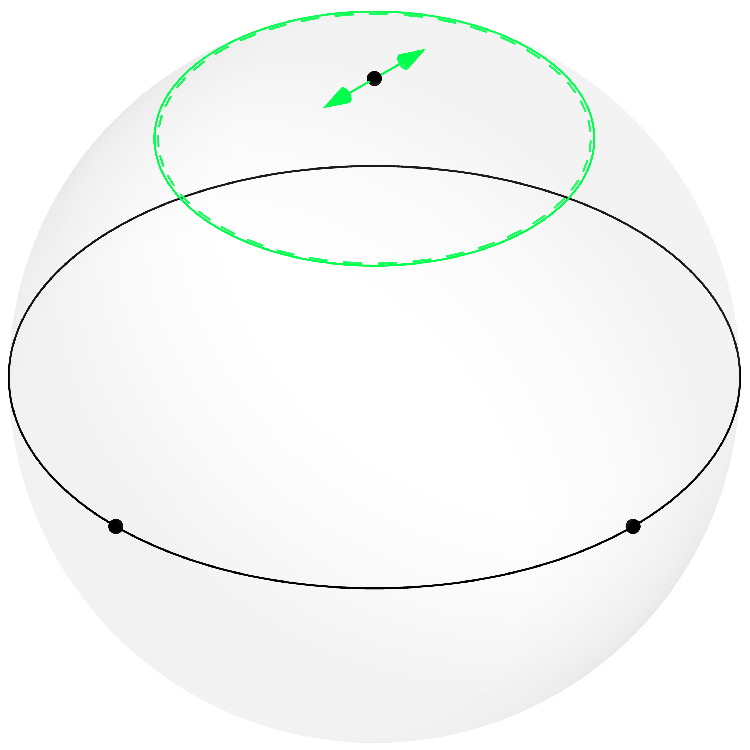
\includegraphics[width=1.0\columnwidth]{pol_illum/scene0.pdf}\\
      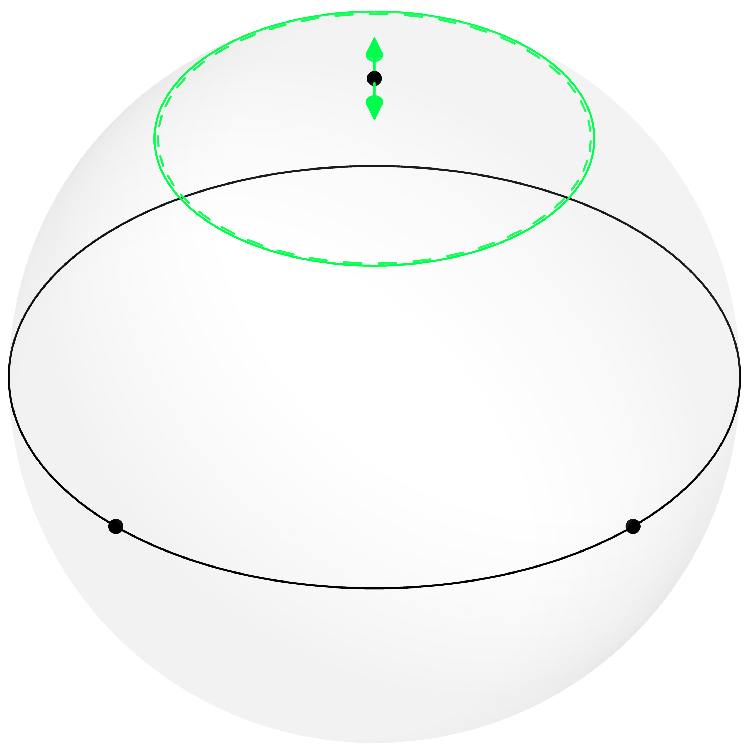
\includegraphics[width=1.0\columnwidth]{pol_illum/scene1.pdf}
    \end{column}
    \begin{column}{0.25\textwidth}
      \centering      
      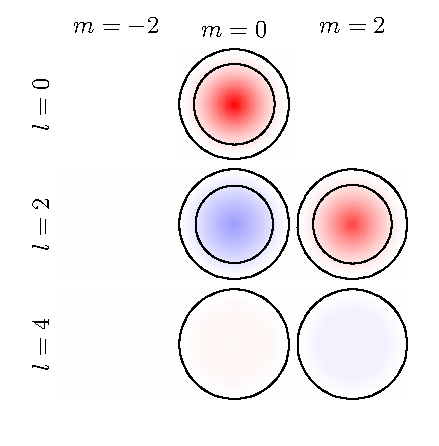
\includegraphics[width=1.0\columnwidth]{pol_illum/otf0.pdf}\\
      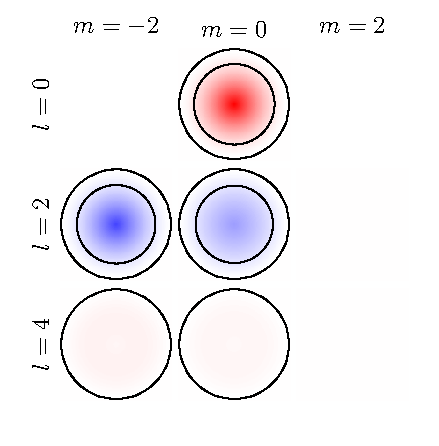
\includegraphics[width=1.0\columnwidth]{pol_illum/otf1.pdf}
    \end{column}
    \begin{column}{0.25\textwidth}
      \centering
      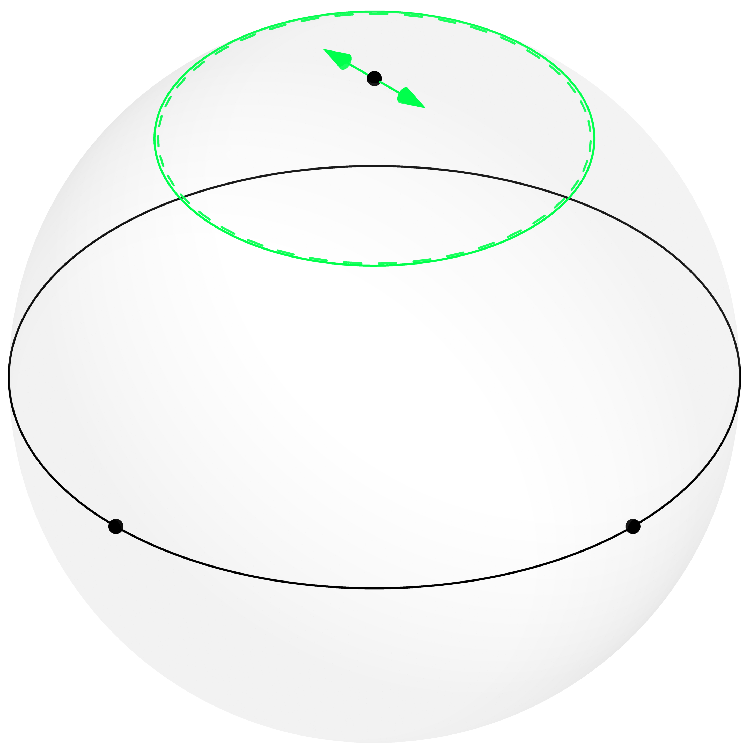
\includegraphics[width=1.0\columnwidth]{pol_illum/scene2.pdf}\\
      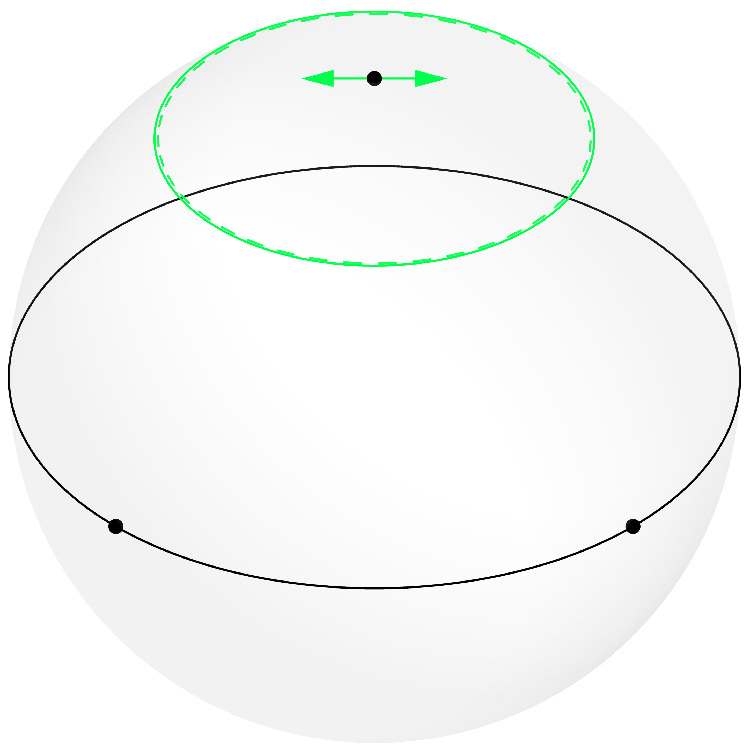
\includegraphics[width=1.0\columnwidth]{pol_illum/scene3.pdf}      
    \end{column}
    \begin{column}{0.25\textwidth}
      \centering
      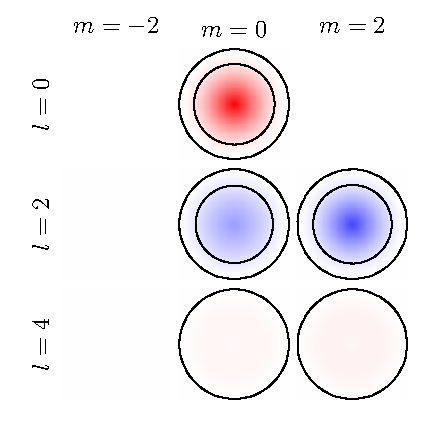
\includegraphics[width=1.0\columnwidth]{pol_illum/otf2.pdf}\\
      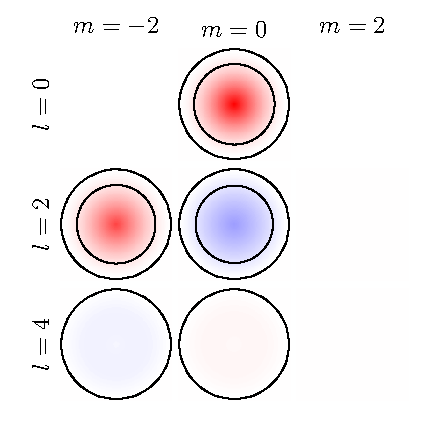
\includegraphics[width=1.0\columnwidth]{pol_illum/otf3.pdf}      
    \end{column}
  \end{columns}
\end{frame}


\begin{frame}[label=sec-1]{4-frame polarized detection OTFs}
  \begin{columns}
    \begin{column}{0.25\textwidth}
      \centering      
      \includegraphics[width=1.0\columnwidth]{pol_detect/scene0.pdf}\\
      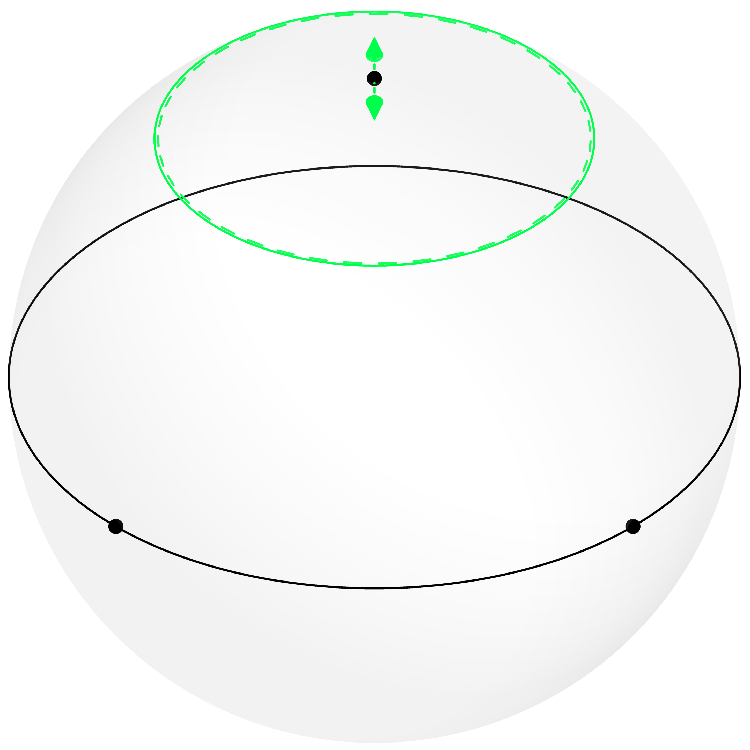
\includegraphics[width=1.0\columnwidth]{pol_detect/scene1.pdf}
    \end{column}
    \begin{column}{0.25\textwidth}
      \centering      
      \includegraphics[width=1.0\columnwidth]{pol_detect/otf0.pdf}\\
      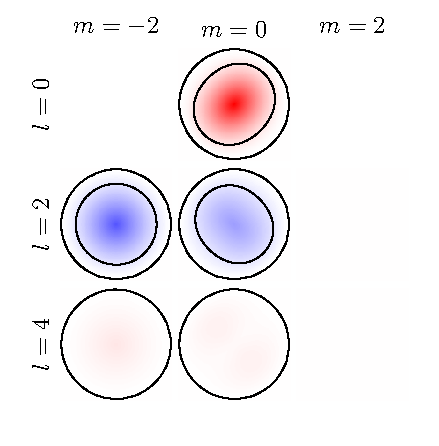
\includegraphics[width=1.0\columnwidth]{pol_detect/otf1.pdf}
    \end{column}
    \begin{column}{0.25\textwidth}
      \centering
      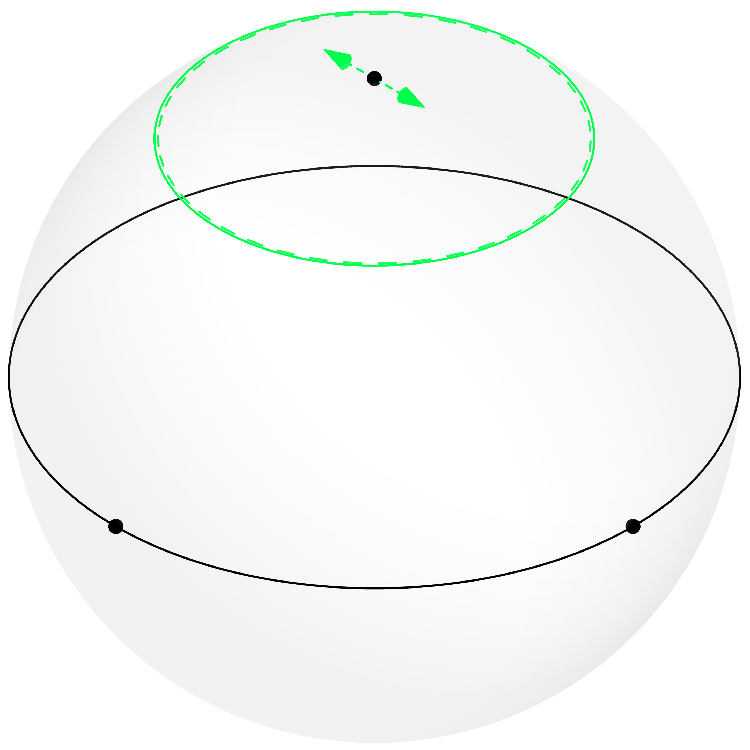
\includegraphics[width=1.0\columnwidth]{pol_detect/scene2.pdf}\\
      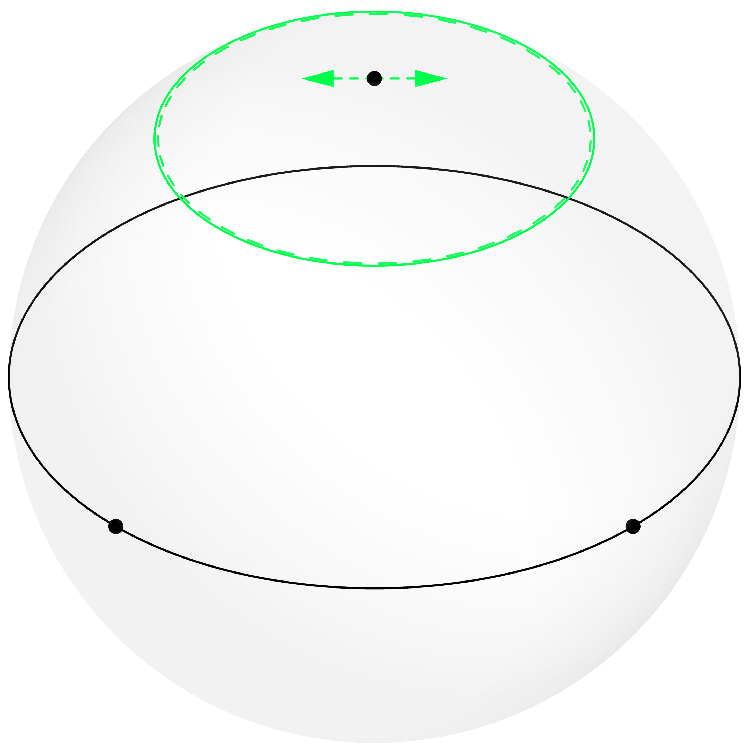
\includegraphics[width=1.0\columnwidth]{pol_detect/scene3.pdf}      
    \end{column}
    \begin{column}{0.25\textwidth}
      \centering
      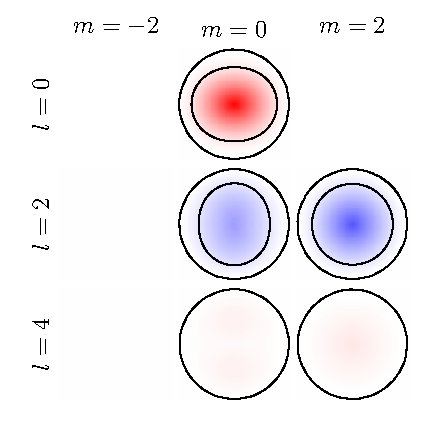
\includegraphics[width=1.0\columnwidth]{pol_detect/otf2.pdf}\\
      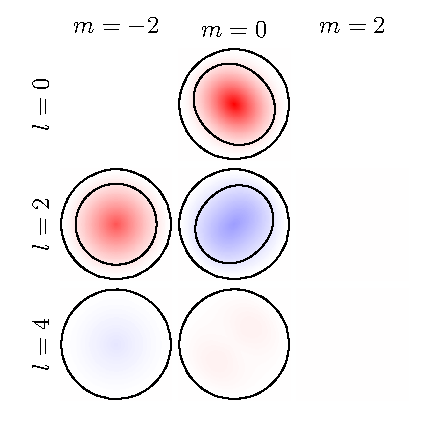
\includegraphics[width=1.0\columnwidth]{pol_detect/otf3.pdf}      
    \end{column}
  \end{columns}
\end{frame}

\begin{frame}[label=sec-1]{3-frame polarized detection OTFs}
  \begin{columns}
    \begin{column}{0.25\textwidth}
      \centering      
      \includegraphics[width=1.0\columnwidth]{pol_detect3/scene0.pdf}\\
      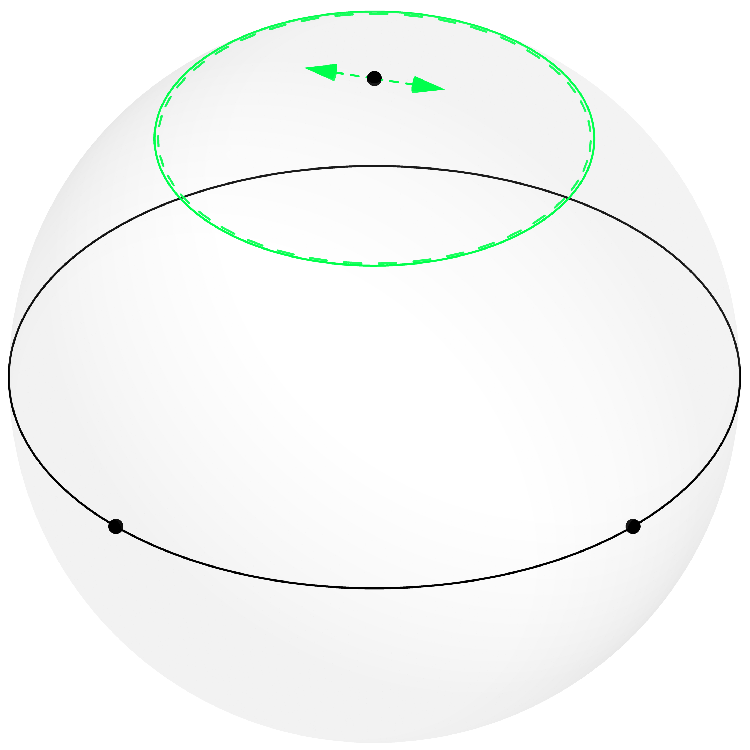
\includegraphics[width=1.0\columnwidth]{pol_detect3/scene1.pdf}
    \end{column}
    \begin{column}{0.25\textwidth}
      \centering      
      \includegraphics[width=1.0\columnwidth]{pol_detect3/otf0.pdf}\\
      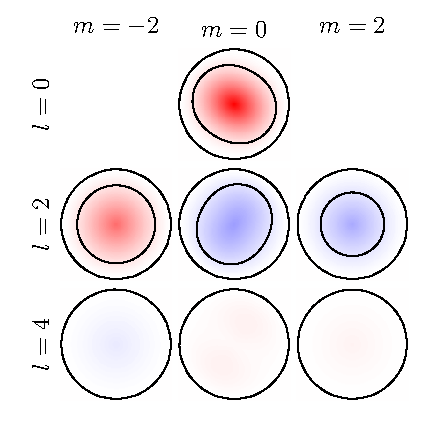
\includegraphics[width=1.0\columnwidth]{pol_detect3/otf1.pdf}
    \end{column}
    \begin{column}{0.25\textwidth}
      \centering
      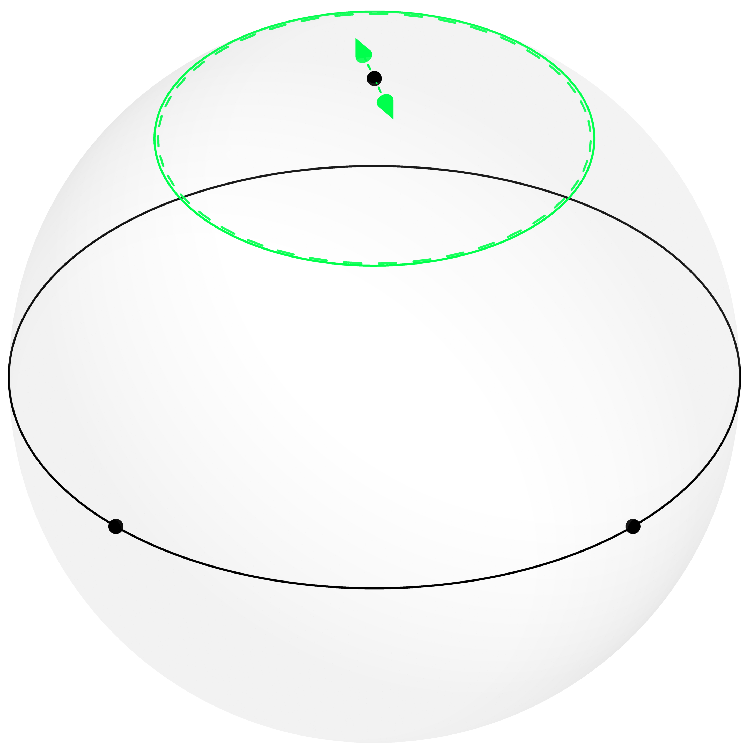
\includegraphics[width=1.0\columnwidth]{pol_detect3/scene2.pdf}\\
    \end{column}
    \begin{column}{0.25\textwidth}
      \centering
      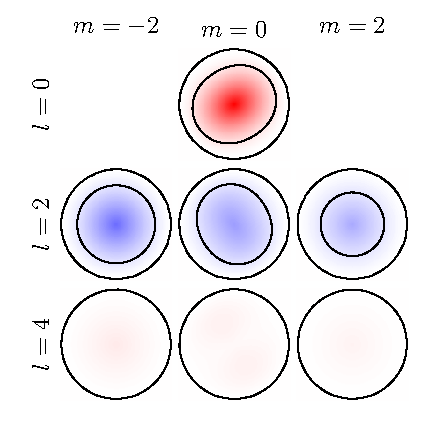
\includegraphics[width=1.0\columnwidth]{pol_detect3/otf2.pdf}\\
    \end{column}
  \end{columns}
\end{frame}

\begin{frame}{Singular system}
  \vspace{-2em}
  \begin{align*}
    \intertext{Forward model:}
    [\mathcal{H}f]_n(\rd{}) = \int_{\mbb{S}^2}d\so{}\int_{\mbb{R}^2}d\ro{}\, h_n(\rd{} -\ro{}, \so{})f(\ro{}, \so{}),\quad  n=1, 2,\ldots,N,
    \end{align*}
    \begin{align*}    
    \intertext{Adjoint:}
    [\mathcal{H}^{\dagger}\mb{g}](\ro{}, \so{}) = \sum_{n=1}^N\int_{\mbb{R}^2}d\mb{r}_{d}\, h_n(\rd{} - \ro{}, \so{})g_n(\rd{}).\label{eq:adj}
    \end{align*}
    \begin{align*}
    \intertext{Eigenvalue problems:}
      \mathcal{H}^{\dagger}\mathcal{H}u_{\bs{\rho},j}(\ro{}, \so{}) &= \mu_{\bs{\rho},j}u_{\bs{\rho},j}(\ro{}, \so{})\\
    \mathcal{H}\mathcal{H}^{\dagger}\mb{v}_{\bs{\rho},j}(\rd{}) &= \mu_{\bs{\rho},j}\mb{v}_{\bs{\rho},j}(\rd{})         
  \end{align*}
\end{frame}



\begin{frame}[label=sec-1]{4-frame polarized illumination singular spectrum}
  \begin{columns}
    \begin{column}{0.25\textwidth}
      \centering
      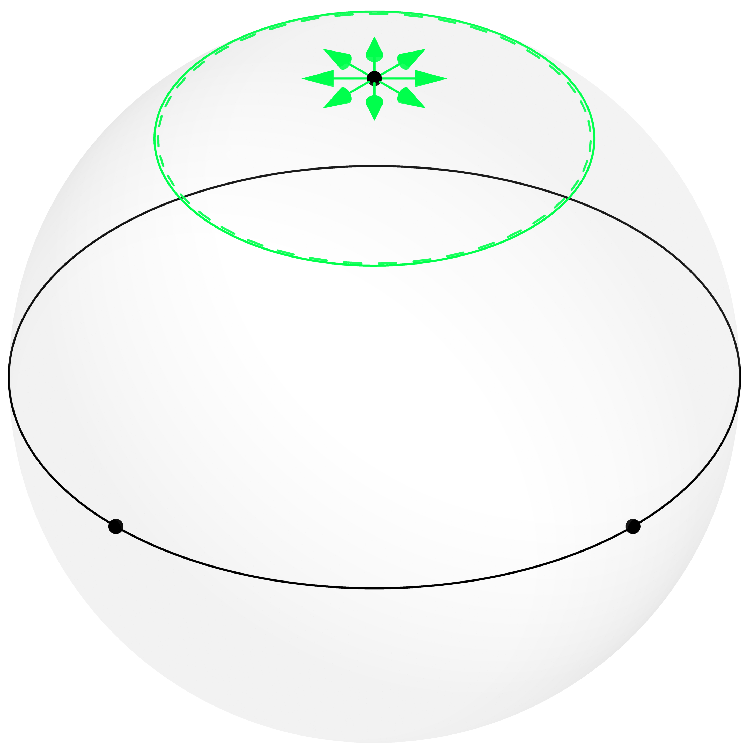
\includegraphics[width=1.0\columnwidth]{pol_illum/scene.pdf}
    \end{column}
    \begin{column}{0.75\textwidth}
      \centering
      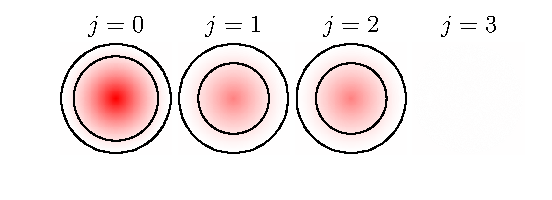
\includegraphics[width=1.0\columnwidth]{pol_illum/svs.pdf}
    \end{column}
  \end{columns}
\end{frame}

\begin{frame}[label=sec-1]{4-frame polarized detection singular spectrum}
  \begin{columns}
    \begin{column}{0.25\textwidth}
      \centering
      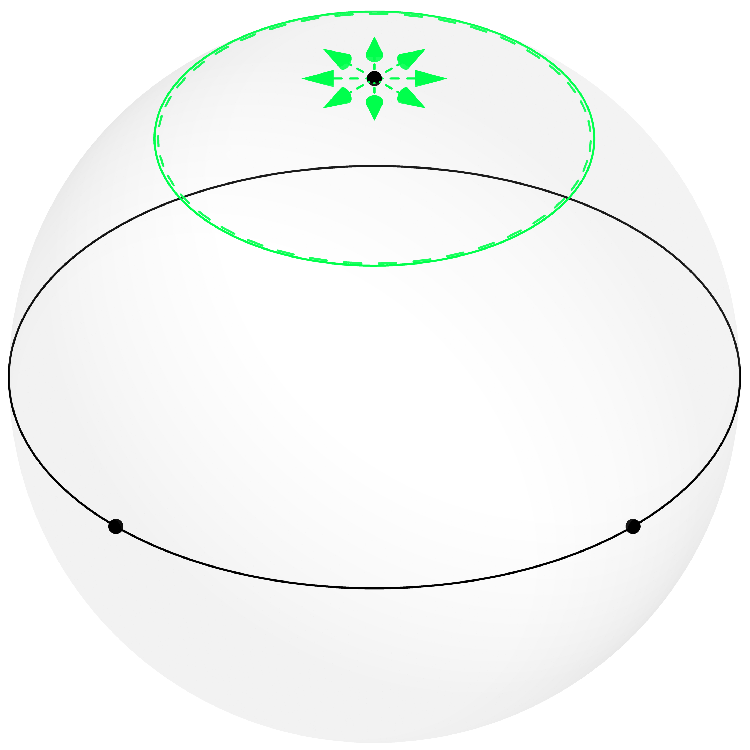
\includegraphics[width=1.0\columnwidth]{pol_detect/scene.pdf}
    \end{column}
    \begin{column}{0.75\textwidth}
      \centering
      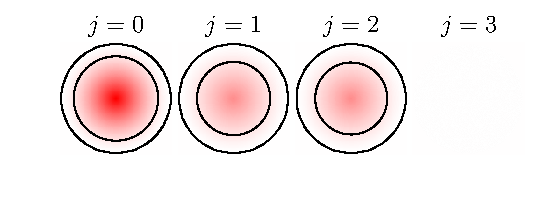
\includegraphics[width=1.0\columnwidth]{pol_detect/svs.pdf}
    \end{column}
  \end{columns}
\end{frame}

\begin{frame}[label=sec-1]{3-frame polarized detection singular spectrum}
  \begin{columns}
    \begin{column}{0.25\textwidth}
      \centering
      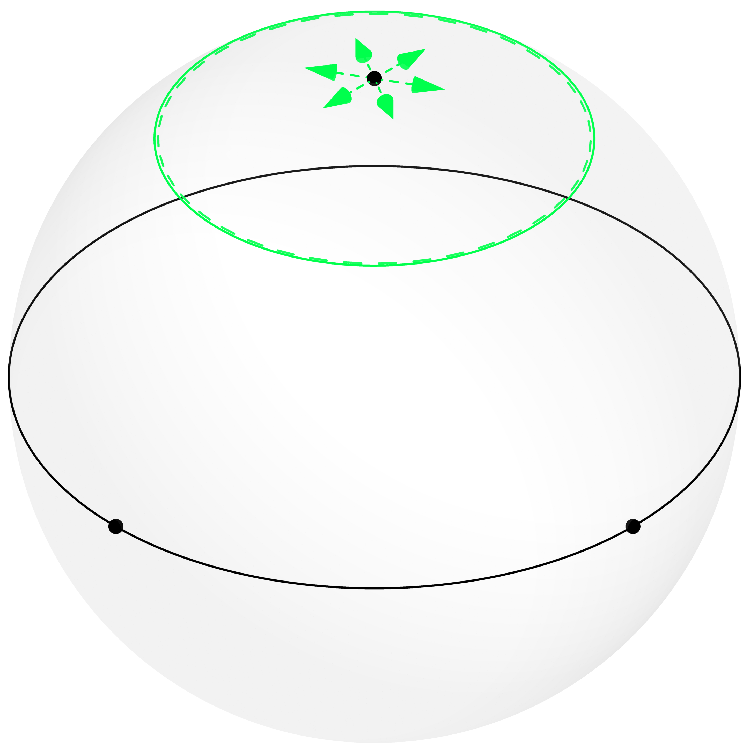
\includegraphics[width=1.0\columnwidth]{pol_detect3/scene.pdf}
    \end{column}
    \begin{column}{0.75\textwidth}
      \centering
      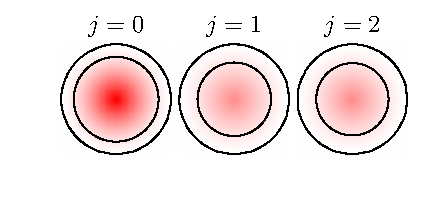
\includegraphics[width=1.0\columnwidth]{pol_detect3/svs.pdf}
    \end{column}
  \end{columns}
\end{frame}


\begin{frame}{More insight from CC-CC model? $\mbb{L}_2(\mbb{R}^2 \times \mbb{S}^2) \rightarrow \mbb{L}_2(\mbb{R}^{2}\times \mbb{S}^1)$}
  \vspace{-2em}
  \begin{align*}
    \intertext{Forward model:}
    [\mathcal{H}f](\rd{}, \hat{\mb{p}}) = \int_{\mbb{S}^2}d\so{}\int_{\mbb{R}^2}d\ro{}\, h(\rd{} -\ro{}, \so{}; \hat{\mb{p}})f(\ro{}, \so{}),
  \end{align*}
    \begin{align*}    
    \intertext{Adjoint:}
    [\mathcal{H}^{\dagger}g](\ro{}, \so{}) = \int_{\mbb{S}^1}d\hat{\mb{p}}\, \int_{\mbb{R}^2}d\mb{r}_{d}\, h(\rd{} - \ro{}, \so{}; \hat{\mb{p}})g(\rd{}, \hat{\mb{p}}).
    \end{align*}
  %   \begin{align*}
  %   \intertext{Eigenvalue problems:}
  %     \mathcal{H}^{\dagger}\mathcal{H}u_{\bs{\rho},j}(\ro{}, \so{}) &= \mu_{\bs{\rho},j}u_{\bs{\rho},j}(\ro{}, \so{})\\
  %   \mathcal{H}\mathcal{H}^{\dagger}\mb{v}_{\bs{\rho},j}(\rd{}) &= \mu_{\bs{\rho},j}\mb{v}_{\bs{\rho},j}(\rd{})         
  % \end{align*}
\end{frame}

  
\end{document}